%%%%%%%%%%%%%%%%%%%%%%%%%%%%%%%%%%%%%%%%%%%%%%%%%%%%%%%%%%%%%%%%%
% Contents: Typesetting Part of LaTeX2e Introduction
% $Id$
%%%%%%%%%%%%%%%%%%%%%%%%%%%%%%%%%%%%%%%%%%%%%%%%%%%%%%%%%%%%%%%%%
\chapter{Typesetting Text}

\begin{intro}
  After reading the previous chapter, you should know about the basic
  stuff of which a \LaTeXe{} document is made. In this chapter I
  will fill in the remaining structure you will need to know in order
  to produce real world material.
\end{intro}

\section{The Structure of Text and Language}
\secby{Hanspeter Schmid}{hanspi@schmid-werren.ch}
The main point of writing a text, is to convey ideas, information, or
knowledge to the reader.  The reader will understand the text better
if these ideas are well-structured, and will see and feel this
structure much better if the typographical form reflects the logical
and semantic structure of the content.

\LaTeX{} is different from other typesetting systems in that you just
have to tell it the logical and semantic structure of a text.  It
then derives the typographical form of the text according to the
``rules'' given in the document class file and in various style files.

The most important text unit in \LaTeX{} (and in typography) is the
\wi{paragraph}.  We call it ``text unit'' because a paragraph is the
typographical form that should reflect one coherent thought, or one idea.
You will learn in the following sections how to force line breaks with
e.g.\ \texttt{\bs\bs}, and paragraph breaks with e.g.\ leaving an empty line
in the source code.  Therefore, if a new thought begins, a new paragraph
should begin, and if not, only line breaks should be used.  If in doubt
about paragraph breaks, think about your text as a conveyor of ideas and
thoughts.  If you have a paragraph break, but the old thought continues, it
should be removed.  If some totally new line of thought occurs in the same
paragraph, then it should be broken.

Most people completely underestimate the importance of well-placed
paragraph breaks.  Many people do not even know what the meaning of
a paragraph break is, or, especially in \LaTeX, introduce paragraph
breaks without knowing it.  The latter mistake is especially easy to
make if equations are used in the text.  Look at the following
examples, and figure out why sometimes empty lines (paragraph breaks)
are used before and after the equation, and sometimes not.  (If you
don't yet understand all commands well enough to understand these
examples, please read this and the following chapter, and then read
this section again.)

\begin{code}
\begin{verbatim}
% Example 1
\ldots when Einstein introduced his formula
\begin{equation}
  e = m \cdot c^2 \; ,
\end{equation}
which is at the same time the most widely known
and the least well understood physical formula.


% Example 2
\ldots from which follows Kirchhoff's current law:
\begin{equation}
  \sum_{k=1}^{n} I_k = 0 \; .
\end{equation}

Kirchhoff's voltage law can be derived \ldots


% Example 3
\ldots which has several advantages.

\begin{equation}
  I_D = I_F - I_R
\end{equation}
is the core of a very different transistor model. \ldots
\end{verbatim}
\end{code}

The next smaller text unit is a sentence.  In English texts, there is
a larger space after a period that ends a sentence than after one
that ends an abbreviation.  \LaTeX{} tries to figure out which one
you wanted to have.  If \LaTeX{} gets it wrong, you must tell it what
you want.  This is explained later in this chapter.

The structuring of text even extends to parts of sentences.  Most
languages have very complicated punctuation rules, but in many
languages (including German and English), you will get almost every
comma right if you remember what it represents: a short stop in the
flow of language.  If you are not sure about where to put a comma,
read the sentence aloud and take a short breath at every comma.  If
this feels awkward at some place, delete that comma; if you feel the
urge to breathe (or make a short stop) at some other place, insert a
comma.

Finally, the paragraphs of a text should also be structured logically
at a higher level, by putting them into chapters, sections,
subsections, and so on.  However, the typographical effect of writing
e.g.\ \verb|\section{The| \texttt{Structure of Text and Language}\verb|}| is
so obvious that it is almost self-evident how these high-level
structures should be used.

\section{Line Breaking and Page Breaking}

\subsection{Justified Paragraphs}

Books are often typeset with each line having the same length.
\LaTeX{} inserts the necessary \wi{line break}s and spaces between words
by optimizing the contents of a whole paragraph. If necessary, it
also hyphenates words that would not fit comfortably on a line.
How the paragraphs are typeset depends on the document class.
Normally the first line of a paragraph is indented, and there is no
additional space between two paragraphs. Refer to section~\ref{parsp}
for more information.

In special cases it might be necessary to order \LaTeX{} to break a
line:
\begin{lscommand}
\ci{\bs} or \ci{newline}
\end{lscommand}
\noindent starts a new line without starting a new paragraph.

\begin{lscommand}
\ci{\bs*}
\end{lscommand}
\noindent additionally prohibits a page break after the forced
line break.

\begin{lscommand}
\ci{newpage}
\end{lscommand}
\noindent starts a new page.

\begin{lscommand}
\ci{linebreak}\verb|[|\emph{n}\verb|]|,
\ci{nolinebreak}\verb|[|\emph{n}\verb|]|,
\ci{pagebreak}\verb|[|\emph{n}\verb|]|,
\ci{nopagebreak}\verb|[|\emph{n}\verb|]|
\end{lscommand}
\noindent suggest places where a break may (or may not) happen. They enable the author to influence their
actions with the optional argument \emph{n}, which can be set to a number
between zero and four. By setting \emph{n} to a value below 4, you leave
\LaTeX{} the option of ignoring your command if the result would look very
bad. Do not confuse these ``break'' commands with the ``new'' commands. Even
when you give a ``break'' command, \LaTeX{} still tries to even out the
right border of the line and the total length of the page, as described in
the next section; this can lead to unpleasant gaps in your text.
If you really want to start a ``new line'' or a ``new page'', then use the
corresponding command. Guess their names!


\LaTeX{} always tries to produce the best line breaks possible. If it
cannot find a way to break the lines in a manner that meets its high
standards, it lets one line stick out on the right of the paragraph.
\LaTeX{} then complains (``\wi{overfull hbox}'') while processing the
input file. This happens most often when \LaTeX{} cannot find a
suitable place to hyphenate a word.\footnote{Although \LaTeX{} gives
  you a warning when that happens (\texttt{Overfull \bs{}hbox}) and displays the
  offending line, such lines are not always easy to find. If you use
  the option \texttt{draft} in the \ci{documentclass} command, these
  lines will be marked with a thick black line on the right margin.}
Instruct \LaTeX{} to lower its standards a little by giving
the \ci{sloppy} command. It prevents such over-long lines by
increasing the inter-word spacing---even if the final output is not
optimal.  In this case a warning (``\wi{underfull hbox}'') is given to
the user.  In most such cases the result doesn't look very good. The
command \ci{fussy} brings \LaTeX{} back to its default behaviour.

\subsection{Hyphenation} \label{hyph}

\LaTeX{} hyphenates words whenever necessary. If the hyphenation
algorithm does not find the correct hyphenation points,
remedy the situation by using the following commands to tell \TeX{}
about the exception.

The command
\begin{lscommand}
\ci{hyphenation}\verb|{|\emph{word list}\verb|}|
\end{lscommand}
\noindent causes the words listed in the argument to be hyphenated only at
the points marked by ``\verb|-|''.  The argument of the command should only
contain words built from normal letters, or rather signs that are considered
to be normal letters by \LaTeX{}. The hyphenation hints are
stored for the language that is active when the hyphenation command
occurs. This means that if you place a hyphenation command into the preamble
of your document it will influence the English language hyphenation. If you
place the command after the \verb|\begin{document}| and you are using some
package for national language support like \pai{polyglossia}, then the hyphenation
hints will be active in the language activated through \pai{polyglossia}.

The example below will allow ``hyphenation'' to be hyphenated as well as
``Hyphenation'', and it prevents ``FORTRAN'', ``Fortran'' and ``fortran''
from being hyphenated at all.  No special characters or symbols are allowed
in the argument.

Example:
\begin{code}
\verb|\hyphenation{FORTRAN Hy-phen-a-tion}|
\end{code}

The command \ci{-} inserts a discretionary hyphen into a word. This
also becomes the only point hyphenation is allowed in this word. This
command is especially useful for words containing special characters
(e.g.\ accented characters), because \LaTeX{} does not automatically
hyphenate words containing special characters.
%\footnote{Unless you are using the new
%\wi{DC fonts}.}.

\begin{example}
I think this is: su\-per\-cal\-%
i\-frag\-i\-lis\-tic\-ex\-pi\-%
al\-i\-do\-cious
\end{example}

Several words can be kept together on one line with the command
\begin{lscommand}
\ci{mbox}\verb|{|\emph{text}\verb|}|
\end{lscommand}
\noindent It causes its argument to be kept together under all circumstances.

\begin{example}
My phone number will change soon.
It will be \mbox{0116 291 2319}.

The parameter
\mbox{\emph{filename}} should
contain the name of the file.
\end{example}

\ci{fbox} is similar to \ci{mbox}, but in addition there will
be a visible box drawn around the content.


\section{Ready-Made Strings}

In some of the examples on the previous pages, you have seen
some very simple \LaTeX{} commands for typesetting special
text strings:

\vspace{2ex}

\noindent
\begin{tabular}{@{}lll@{}}
Command&Example&Description\\
\hline
\ci{today} & \today   & Current date\\
\ci{TeX} & \TeX       & Your favorite typesetter\\
\ci{LaTeX} & \LaTeX   & The Name of the Game\\
\ci{LaTeXe} & \LaTeXe & The current incarnation\\
\end{tabular}

\section{Special Characters and Symbols}

\subsection{Quotation Marks}

You should \emph{not} use the \verb|"| for \wi{quotation marks}
\index{""@\texttt{""}} as you would on a typewriter.  In publishing
there are special opening and closing quotation marks.  In \LaTeX{},
use two~\textasciigrave~(grave accent) for opening quotation marks and
two~\textquotesingle~(vertical quote) for closing quotation marks. For single
quotes you use just one of each.
\begin{example}
``Please press the `x' key.''
\end{example}
Yes I know the rendering is not ideal, it's really a back-tick or grave accent
(\textasciigrave) for
opening quotes and vertical quote (\textquotesingle) for closing, despite what the font chosen might suggest.

\subsection{Dashes and Hyphens}

\LaTeX{} knows four kinds of \wi{dash}es. Access three of
them with different number of consecutive dashes. The fourth sign
is actually not a dash at all---it is the mathematical minus sign: \index{-}
\index{--} \index{---} \index{-@$-$} \index{mathematical!minus}

\begin{example}
daughter-in-law, X-rated\\
pages 13--67\\
yes---or no? \\
$0$, $1$ and $-1$
\end{example}
The names for these dashes are:
`-' \wi{hyphen}, `--' \wi{en-dash}, `---' \wi{em-dash} and
`$-$' \wi{minus sign}.

\subsection{Tilde ($\sim$)}
\index{URL link}\index{tilde}
A character often seen in web addresses is the tilde. To generate
this in \LaTeX{} use \verb|\~{}| but the result (\~{}) is not really
what you want. Try this instead:

\begin{example}
http://www.rich.edu/\~{}bush \\
http://www.clever.edu/$\sim$demo
\end{example}

\subsection{Slash (/)}
\index{Slash}
In order to typeset a slash between two words, one can simply type e.g.\
\texttt{read/write}, but this makes \LaTeX{} treat the two words as one.
Hyphenation is disabled for these two words, so there may be `overfull'
errors.  To overcome this, use \ci{slash}.  For example type
`\verb|read\slash write|' which allows hyphenation.  But normal `\texttt{/}'
character may be still used for ratios or units, e.g.\ \texttt{5 MB/s}.

\subsection{Degree Symbol \texorpdfstring{($\circ$)}{}}

Printing the \wi{degree symbol} in pure \LaTeX{}.

\begin{example}
It's $-30\,^{\circ}\mathrm{C}$.
I will soon start to
super-conduct.
\end{example}

The \pai{textcomp} package makes the degree symbol also available as
\ci{textdegree} or in combination with the C by using the \ci{textcelsius}.

\begin{example}
30 \textcelsius{} is
86 \textdegree{}F.
\end{example}

\subsection{The Euro Currency Symbol \texorpdfstring{(\officialeuro)}{}}

When writing about money these days, you need the Euro symbol. Many current
fonts contain a Euro symbol. After loading the \pai{textcomp} package in the preamble of your document
\begin{lscommand}
\ci{usepackage}\verb|{textcomp}|
\end{lscommand}
use the command
\begin{lscommand}
\ci{texteuro}
\end{lscommand}
to access it.

If your font does not provide its own Euro symbol or if you do not like the
font's Euro symbol, you have two more choices:

First the \pai{eurosym} package. It provides the official Euro symbol:
\begin{lscommand}
\ci{usepackage}\verb|[|\emph{official}\verb|]{eurosym}|
\end{lscommand}
If you prefer a Euro symbol that matches your font, use the option
\texttt{gen} in place of the \texttt{official} option.

%If the Adobe Eurofonts are installed on your system (they are available for
%free from \url{ftp://ftp.adobe.com/pub/adobe/type/win/all}) you can use
%either the package \pai{europs} and the command \ci{EUR} (for a Euro symbol
%that matches the current font).
% does not work
% or the package
% \pai{eurosans} and the command \ci{euro} (for the ``official Euro'').

%The \pai{marvosym} package also provides many different symbols, including a
%Euro, under the name \ci{EURtm}. Its disadvantage is that it does not provide
%slanted and bold variants of the Euro symbol.

\begin{table}[!htbp]
\caption{A bag full of Euro symbols} \label{eurosymb}
\begin{lined}{10cm}
\begin{tabular}{llccc}
LM+textcomp  &\verb+\texteuro+ & \huge\texteuro &\huge\sffamily\texteuro
                                                &\huge\ttfamily\texteuro\\
eurosym      &\verb+\euro+ & \huge\officialeuro &\huge\sffamily\officialeuro
                                                &\huge\ttfamily\officialeuro\\
$[$gen$]$eurosym &\verb+\euro+ & \huge\geneuro  &\huge\sffamily\geneuro
                                                &\huge\ttfamily\geneuro\\
%europs       &\verb+\EUR + & \huge\EURtm        &\huge\EURhv
%                                                &\huge\EURcr\\
%eurosans     &\verb+\euro+ & \huge\EUROSANS  &\huge\sffamily\EUROSANS
%                                             & \huge\ttfamily\EUROSANS \\
%marvosym     &\verb+\EURtm+  & \huge\mvchr101  &\huge\mvchr101
%                                               &\huge\mvchr101
\end{tabular}
\medskip
\end{lined}
\end{table}

\subsection{Ellipsis (\texorpdfstring{\ldots}{...})}

On a typewriter, a \wi{comma} or a \wi{period} takes the same amount of
space as any other letter. In book printing, these characters occupy
only a little space and are set very close to the preceding letter.
Therefore, entering `\wi{ellipsis}' by just typing three
dots would produce the wrong result. Instead, there is a special
command for these dots. It is called

\begin{lscommand}
\ci{ldots} (low dots)
\end{lscommand}
\index{...@\ldots}


\begin{example}
Not like this ... but like this:\\
New York, Tokyo, Budapest, \ldots
\end{example}

\subsection{Ligatures}

Some letter combinations are typeset not just by setting the
different letters one after the other, but by actually using special
symbols.
\begin{code}
{\large ff fi fl ffi\ldots}\quad
instead of\quad {\large f{}f f{}i f{}l f{}f{}i \ldots}
\end{code}
These so-called \wi{ligature}s can be prohibited by inserting an \ci{mbox}\verb|{}|
between the two letters in question. This might be necessary with
words built from two words.

\begin{example}
\Large Not shelfful\\
but shelf\mbox{}ful
\end{example}

\subsection{Accents and Special Characters}

\LaTeX{} supports the use of \wi{accent}s and \wi{special character}s
from many languages. Table~\ref{accents} shows all sorts of accents
being applied to the letter o. Naturally other letters work too.

To place an accent on top of an i or a j, its dots have to be
removed. This is accomplished by typing \verb|\i| and \verb|\j|.

\begin{example}
H\^otel, na\"\i ve, \'el\`eve,\\
sm\o rrebr\o d, !`Se\~norita!,\\
Sch\"onbrunner Schlo\ss{}
Stra\ss e
\end{example}

\begin{table}[!hbp]
\caption{Accents and Special Characters.} \label{accents}
\begin{lined}{10cm}
\begin{tabular}{*4{cl}}
\mstA{\`o} & \mstA{\'o} & \mstA{\^o} & \mstA{\~o} \\
\mstA{\=o} & \mstA{\.o} & \mstA{\"o} & \mstB{\c}{c}\\[6pt]
\mstB{\u}{o} & \mstB{\v}{o} & \mstB{\H}{o} & \mstB{\c}{o} \\
\mstB{\d}{o} & \mstB{\b}{o} & \mstB{\t}{oo} \\[6pt]
\mstA{\oe}  &  \mstA{\OE} & \mstA{\ae} & \mstA{\AE} \\
\mstA{\aa} &  \mstA{\AA} \\[6pt]
\mstA{\o}  & \mstA{\O} & \mstA{\l} & \mstA{\L} \\
\mstA{\i}  & \mstA{\j} & !` & \verb|!`| & ?` & \verb|?`|
\end{tabular}
\index{dotless \i{} and \j}\index{Scandinavian letters}
\index{ae@\ae}\index{umlaut}\index{grave}\index{acute}
\index{oe@\oe}\index{aa@\aa}

\bigskip
\end{lined}
\end{table}

\section{International Language Support}
\secby{Axel Kielhorn}{A.Kielhorn@web.de}%
\index{international} When you write documents in \wi{language}s
other than English, there are three areas where \LaTeX{} has to be
configured appropriately:

\begin{enumerate}
\item All automatically generated text strings\footnote{Table of
    Contents, List of Figures, \ldots} have to be adapted to the new
  language.
\item \LaTeX{} needs to know the hyphenation rules for the current language.
\item Language specific typographic rules. In French for example, there is a
  mandatory space before each colon character (:).
\end{enumerate}

Also entering text in your language of choice might be a bit cumbersome using all the
commands from figure~\ref{accents}. To overcome this problem, until recently you had to delve
deep into the abyss of language specific encodings both for input as well as fonts. These days,
with modern \TeX{} engines speaking UTF-8 natively, these problems have relaxed considerably.

The package \pai{polyglossia}\cite{polyglossia} is a replacement for
venerable \pai{babel} package. It takes care of the hyphenation patterns and automatically
generated text strings in your documents.

The package \pai{fontspec}\cite{fontspec} handles font loading for
\hologo{XeLaTeX} and \hologo{LuaTeX}. The default font is Latin Modern
Roman.

\subsection{Polyglossia Usage}

Depending on the \TeX{} engine you use slighly different commands are
necessary in the preamble of your document to properly enable multilingual
processing. Figure~\ref{allinone} on page~\pageref{allinone} shows a sample preamble that takes care of all the necessary settings.

\begin{figure}[!bp]
\begin{lined}{10cm}
\begin{verbatim}
\usepackage{iftex}
\ifXeTeX
   \usepackage{fontspec}
\else
   \usepackage{luatextra}
\fi
\defaultfontfeatures{Ligatures=TeX}
\usepackage{polyglossia}
\end{verbatim}
\end{lined}
\caption[All in one preamble]{All in one preamble that takes care of \hologo{LuaLaTeX} and \hologo{XeLaTeX}} \label{allinone}
\end{figure}

So far there has been no advantage to using a Unicode \hologo{TeX} engine.
This changes when we leave the Latin script and move to a more interesting
language like Greek or Russian.  With a Unicode based system, you can
simply\footnote{For small values of simple.} enter the native characters in your
editor and \hologo{TeX} will understand them.

Writing in different languages is easy, just specify the languages in the
preamble. This example uses the \pai{csquotes} package which generates
the right kind of quotes according to the language you are writing in. Note
that it needs to be loaded \emph{before} loading the language support.

\begin{lscommand}
\verb|\usepackage[autostyle=true]{csquotes}|\\
\verb|\setdefaultlanguage{english}|\\
\verb|\setotherlanguage{german}|
\end{lscommand}
%
To write a paragraph in German, you can use the German environment:

\begin{example}
English text.
\begin{german}
Deutscher \enquote{Text}.
\end{german}
More English \enquote{text}.
\end{example}

If you just need a word in a foreign language you can use the
\verb|\text|\emph{language} command:

\begin{example}
Did you know that
\textgerman{Gesundheit} is
actually a German word.
\end{example}

This may look unnecessary since the only advantage is a correct hyphenation,
but when the second language is a little bit more exotic it will be worth
the effort.

Sometimes the font used in the main document does not contain glyphs that
are required in the second language. Latin Modern for example does not contain
Cyrillic letters. The solution is to define a font that will be used for
that language. Whenever a new language is activated, \pai{polyglossia} will
first check whether a font has been defined for that language. If you are happy with the computer modern font, you may want to try the \enquote{Computer Modern Unicode} font by adding the following commands to the preamble of your document.

\medskip\noindent For \hologo{LuaLaTeX} it is pretty simple
\begin{verbatim}
\setmainfont{CMU Serif}
\setsansfont{CMU Sans Serif}
\setmonofont{CMU Typewriter Text}
\end{verbatim}
\noindent For \hologo{XeLaTeX} you have to be a bit more explicit:
\begin{verbatim}
\setmainfont{cmun}[
   Extension=.otf,UprightFont=*rm,ItalicFont=*ti,
   BoldFont=*bx,BoldItalicFont=*bi,
 ]
 \setsansfont{cmun}[
   Extension=.otf,UprightFont=*ss,ItalicFont=*si,
   BoldFont=*sx,BoldItalicFont=*so,
 ]
 \setmonofont{cmun}[
   Extension=.otf,UprightFont=*btl,ItalicFont=*bto,
   BoldFont=*tb,BoldItalicFont=*tx,
 ]
\end{verbatim}

With the appropriate fonts loaded, you can now write:

\begin{example}
\textrussian{Правда} is
a russian newspaper.
\textgreek{ἀλήθεια} is truth
or disclosure in philosophy
\end{example}

The package \pai{xgreek}\index{Greek}\cite{xgreek} offers support for
writing either ancient or modern (monotonic or polytonic) greek.

\subsubsection{Right to Left (RTL) languages.}

Some languages are written left to right, others are written right to
left(RTL). \pai{polyglossia} needs the \pai{bidi}\cite{bidi}
package\footnote{\texttt{bidi} does not support \hologo{LuaTeX}.} in order
to support RTL languages. The \pai{bidi} package should be the last package
you load, even after \pai{hyperref} which is usually the last package.
(Since \pai{polyglossia} loads \pai{bidi} this means that \pai{polyglossia}
should be the last package loaded.)

The package \pai{xepersian}\index{Persian}\cite{xepersian} offers support
for the Persian language. It supplies Persian \LaTeX-commands that allows
you to enter commands like \verb|\section| in Persian, which makes this
really attractive to native speakers. \pai{xepersian} is the only package
that supports kashida\index{kashida} with \hologo{XeLaTeX}. A package for
Syriac which uses a similar algorithm is under development.

The IranNastaliq font provided by the SCICT\footnote{Supreme Council of
Information and Communication Technology} is available at their website
\url{http://www.scict.ir/Portal/Home/Default.aspx}.

The \pai{arabxetex}\cite{arabxetex} package supports several languages with
an Arabic script:

\begin{itemize}
\item arab (Arabic)\index{Arabic}
\item persian\index{Persian}
\item urdu\index{Urdu}
\item sindhi\index{Sindhi}
\item pashto\index{Pashto}
\item ottoman (turk)\index{Ottoman}\index{Turkish}
\item kurdish\index{Kurdish}
\item kashmiri\index{Kashmiri}
\item malay (jawi)\index{Malay}\index{Jawi}
\item uighur\index{Uighur}
\end{itemize}

It offers a font mapping that enables \hologo{XeLaTeX} to process input
using the Arab\TeX\ ASCII transcription.

Fonts that support several Arabic laguages are offered by the
IRMUG\footnote{Iranian Mac User Group} at
\url{http://wiki.irmug.org/index.php/X_Series_2}.

There is no package available for Hebrew\index{Hebrew} because none is
needed. The Hebrew support in \pai{polyglossia} should be sufficient. But
you do need a suitable font with real Unicode Hebrew. SBL Hebrew is free for
non-commercial use and available at
\url{http://www.sbl-site.org/educational/biblicalfonts.aspx}. Another font
available under the Open Font License is Ezra SIL, available at
\url{http://www.sil.org/computing/catalog/show_software.asp?id=76}.

Remember to select the correct script:

\begin{lscommand}
\verb|\newfontfamily\hebrewfont[Script=Hebrew]{SBL Hebrew}| \\
\verb|\newfontfamily\hebrewfont[Script=Hebrew]{Ezra SIL}|
\end{lscommand}


\subsubsection{Chinese, Japanese and Korean (CJK)}
\index{Chinese}\index{Japanese}\index{Korean}

The package \pai{xeCJK}\cite{xecjk} takes care of font selection and
punctuation for these languages.

\section{The Space Between Words}

To get a straight right margin in the output, \LaTeX{} inserts varying
amounts of space between the words. It inserts slightly more space at
the end of a sentence, as this makes the text more readable.  \LaTeX{}
assumes that sentences end with periods, question marks or exclamation
marks. If a period follows an uppercase letter, this is not taken as a
sentence ending, since periods after uppercase letters normally occur in
abbreviations.

Any exception from these assumptions has to be specified by the
author. A backslash in front of a space generates a space that will
not be enlarged. A tilde~`\verb|~|' character generates a space that cannot be
enlarged and additionally prohibits a line break. The command
\verb|\@| in front of a period specifies that this period terminates a
sentence even when it follows an uppercase letter.
\cih{"@} \index{~@ \verb.~.} \index{tilde@tilde ( \verb.~.)}
\index{., space after}

\begin{example}
Mr.~Smith was happy to see her\\
cf.~Fig.~5\\
I like BASIC\@. What about you?
\end{example}

The additional space after periods can be disabled with the command
\begin{lscommand}
\ci{frenchspacing}
\end{lscommand}
\noindent which tells \LaTeX{} \emph{not} to insert more space after a
period than after an ordinary character. This is very common in
non-English languages, except bibliographies. If you use
\ci{frenchspacing}, the command \verb|\@| is not necessary.

\section{Titles, Chapters, and Sections}

To help the reader find his or her way through your work, you should
divide it into chapters, sections, and subsections.  \LaTeX{} supports
this with special commands that take the section title as their
argument.  It is up to you to use them in the correct order.

The following sectioning commands are available for the
\texttt{article} class: \nopagebreak

\begin{lscommand}
\ci{section}\verb|{...}|\\
\ci{subsection}\verb|{...}|\\
\ci{subsubsection}\verb|{...}|\\
\ci{paragraph}\verb|{...}|\\
\ci{subparagraph}\verb|{...}|
\end{lscommand}

If you want to split your document into parts without influencing the
section or chapter numbering use
\begin{lscommand}
\ci{part}\verb|{...}|
\end{lscommand}

When you work with the \texttt{report} or \texttt{book} class,
an additional top-level sectioning command becomes available
\begin{lscommand}
\ci{chapter}\verb|{...}|
\end{lscommand}

As the \texttt{article} class does not know about chapters, it is quite easy
to add articles as chapters to a book.
The spacing between sections, the numbering and the font size of the
titles will be set automatically by \LaTeX.

Two of the sectioning commands are a bit special:
\begin{itemize}
\item The \ci{part} command does
  not influence the numbering sequence of chapters.
\item The \ci{appendix} command does not take an argument. It just
  changes the chapter numbering to letters.\footnote{For the article
    style it changes the section numbering.}
\end{itemize}

\LaTeX{} creates a table of contents by taking the section headings
and page numbers from the last compile cycle of the document. The command
\begin{lscommand}
\ci{tableofcontents}
\end{lscommand}
\noindent expands to a table of contents at the place it
is issued. A new
document has to be compiled (``\LaTeX ed'') twice to get a
correct \wi{table of contents}. Sometimes it might be
necessary to compile the document a third time. \LaTeX{} will tell you
when this is necessary.

All sectioning commands listed above also exist as ``starred''
versions.  A ``starred'' version of a command is built by adding a
star \verb|*| after the command name.  This generates section headings
that do not show up in the table of contents and are not
numbered. The command \verb|\section{Help}|, for example, would become
\verb|\section*{Help}|.

Normally the section headings show up in the table of contents exactly
as they are entered in the text. Sometimes this is not possible,
because the heading is too long to fit into the table of contents. The
entry for the table of contents can then be specified as an
optional argument in front of the actual heading.

\begin{code}
\verb|\chapter[Title for the table of contents]{A long|\\
\verb|    and especially boring title, shown in the text}|
\end{code}

The \wi{title} of the whole document is generated by issuing a
\begin{lscommand}
\ci{maketitle}
\end{lscommand}
\noindent command. The contents of the title have to be defined by the commands
\begin{lscommand}
\ci{title}\verb|{...}|, \ci{author}\verb|{...}|
and optionally \ci{date}\verb|{...}|
\end{lscommand}
\noindent before calling \verb|\maketitle|. In the argument to \ci{author}, you can supply several names separated by \ci{and} commands.

An example of some of the commands mentioned above can be found in
Figure~\ref{document} on page~\pageref{document}.

Apart from the sectioning commands explained above, \LaTeXe{}
introduced three additional commands for use with the \verb|book| class.
They are useful for dividing your publication. The commands alter
chapter headings and page numbering to work as you would expect in
a book:
\begin{description}
\item[\ci{frontmatter}] should be the very first command after
  the start of the document body (\verb|\begin{document}|). It will switch page numbering to Roman
    numerals and sections will be non-enumerated as if you were using
    the starred sectioning commands (eg \verb|\chapter*{Preface}|)
    but the sections will still show up in the table of contents.
\item[\ci{mainmatter}] comes right before the first chapter of
  the book. It turns on Arabic page numbering and restarts the page
  counter.
\item[\ci{appendix}] marks the start of additional material in your
  book. After this command chapters will be numbered with letters.
\item[\ci{backmatter}] should be inserted before the very last items
  in your book, such as the bibliography and the index. In the standard
  document classes, this has no visual effect.
\end{description}


\section{Cross References}

In books, reports and articles, there are often
\wi{cross-references} to figures, tables and special segments of text.
\LaTeX{} provides the following commands for cross referencing
\begin{lscommand}
\ci{label}\verb|{|\emph{marker}\verb|}|, \ci{ref}\verb|{|\emph{marker}\verb|}|
and \ci{pageref}\verb|{|\emph{marker}\verb|}|
\end{lscommand}
\noindent where \emph{marker} is an identifier chosen by the user. \LaTeX{}
replaces \verb|\ref| by the number of the section, subsection, figure,
table, or theorem after which the corresponding \verb|\label| command
was issued. \verb|\pageref| prints the page number of the
page where the \verb|\label| command occurred.\footnote{Note that these commands
  are not aware of what they refer to. \ci{label} just saves the last
  automatically generated number.} As with section titles and page numbers for the table of contents,
the numbers from the previous compile cycle are used.


\begin{example}
A reference to this subsection
\label{sec:this} looks like:
``see section~\ref{sec:this} on
page~\pageref{sec:this}.''
\end{example}

\section{Footnotes}
With the command
\begin{lscommand}
\ci{footnote}\verb|{|\emph{footnote text}\verb|}|
\end{lscommand}
\noindent a footnote is printed at the foot of the current page.  Footnotes
should always be put\footnote{``put'' is one of the most common
  English words.} after the word or sentence they refer to. Footnotes
referring to a sentence or part of it should therefore be put after
the comma or period.\footnote{Note that footnotes
  distract the reader from the main body of your document. After all,
  everybody reads the footnotes---we are a curious species, so why not
  just integrate everything you want to say into the body of the
  document?\footnotemark}
\footnotetext{A guidepost doesn't necessarily go where it's pointing to :-).}

\begin{example}
Footnotes\footnote{This is
  a footnote.} are often used
by people using \LaTeX.
\end{example}

\section{Emphasized Words}

If a text is typed using a typewriter, important words are
  \texttt{emphasized by \underline{underlining} them.}
\begin{lscommand}
\ci{underline}\verb|{|\emph{text}\verb|}|
\end{lscommand}
In printed books,
however, words are emphasized by typesetting them in an \emph{italic}
font.  As an author you shouldn't care either way. The important bit is, to tell \LaTeX{} that a
particular bit of text is important and should be emphasized. Hence the command
\begin{lscommand}
\ci{emph}\verb|{|\emph{text}\verb|}|
\end{lscommand}
\noindent to emphasize text. What the command actually does with
its argument depends on the context:

\begin{example}
\emph{If you use
  emphasizing inside a piece
  of emphasized text, then
  \LaTeX{} uses the
  \emph{normal} font for
  emphasizing.}
\end{example}

If you want control over font and font size, section \ref{sec:fontsize} on
page \pageref{sec:fontsize} might provide some inspiration.

\section{Environments} \label{env}

% To typeset special purpose text, \LaTeX{} defines many different
% \wi{environment}s for all sorts of formatting:
\begin{lscommand}
\ci{begin}\verb|{|\emph{environment}\verb|}|\quad
   \emph{text}\quad
\ci{end}\verb|{|\emph{environment}\verb|}|
\end{lscommand}
\noindent Where \emph{environment} is the name of the environment. Environments can be
nested within each other as long as the correct nesting order is
maintained.
\begin{code}
\verb|\begin{aaa}...\begin{bbb}...\end{bbb}...\end{aaa}|
\end{code}

\noindent In the following sections all important environments are explained.

\subsection{Itemize, Enumerate, and Description}

The \ei{itemize} environment is suitable for simple lists, the
\ei{enumerate} environment for enumerated lists, and the
\ei{description} environment for descriptions.
\cih{item}

\begin{example}
\flushleft
\begin{enumerate}
\item You can nest the list
environments to your taste:
\begin{itemize}
\item But it might start to
look silly.
\item[-] With a dash.
\end{itemize}
\item Therefore remember:
\begin{description}
\item[Stupid] things will not
become smart because they are
in a list.
\item[Smart] things, though,
can be presented beautifully
in a list.
\end{description}
\end{enumerate}
\end{example}

\subsection{Flushleft, Flushright, and Center}

The environments \ei{flushleft} and \ei{flushright} generate
paragraphs that are either left- or \wi{right-aligned}. \index{left
  aligned} The \ei{center} environment generates centred text. If you
do not issue \ci{\bs} to specify line breaks, \LaTeX{} will
automatically determine line breaks.

\begin{example}
\begin{flushleft}
This text is\\ left-aligned.
\LaTeX{} is not trying to make
each line the same length.
\end{flushleft}
\end{example}

\begin{example}
\begin{flushright}
This text is right-\\aligned.
\LaTeX{} is not trying to make
each line the same length.
\end{flushright}
\end{example}

\begin{example}
\begin{center}
At the centre\\of the earth
\end{center}
\end{example}

\subsection{Quote, Quotation, and Verse}

The \ei{quote} environment is useful for quotes, important phrases and
examples.

\begin{example}
A typographical rule of thumb
for the line length is:
\begin{quote}
On average, no line should
be longer than 66 characters.
\end{quote}
This is why \LaTeX{} pages have
such large borders by default
and also why multicolumn print
is used in newspapers.
\end{example}

There are two similar environments: the \ei{quotation} and the
\ei{verse} environments. The \texttt{quotation} environment is useful
for longer quotes going over several paragraphs, because it indents the
first line of each paragraph. The \texttt{verse} environment is useful for poems
where the line breaks are important. The lines are separated by
issuing a \ci{\bs} at the end of a line and an empty line after each
verse.


\begin{example}
I know only one English poem by
heart. It is about Humpty Dumpty.
\begin{flushleft}
\begin{verse}
Humpty Dumpty sat on a wall:\\
Humpty Dumpty had a great fall.\\
All the King's horses and all
the King's men\\
Couldn't put Humpty together
again.
\end{verse}
\end{flushleft}
\end{example}

\subsection{Abstract}

In scientific publications it is customary to start with an abstract which
gives the reader a quick overview of what to expect. \LaTeX{} provides the
\ei{abstract} environment for this purpose. Normally \ei{abstract} is used
in documents typeset with the article document class.

\newenvironment{abstract}%
        {\begin{center}\begin{small}\begin{minipage}{0.8\textwidth}}%
        {\end{minipage}\end{small}\end{center}}
\begin{example}
\begin{abstract}
The abstract abstract.
\end{abstract}
\end{example}

\subsection{Printing Verbatim}

Text that is enclosed between \verb|\begin{|\ei{verbatim}\verb|}| and
\verb|\end{verbatim}| will be directly printed, as if typed on a
typewriter, with all line breaks and spaces, without any \LaTeX{}
command being executed.

Within a paragraph, similar behavior can be accessed with
\begin{lscommand}
\ci{verb}\verb|+|\emph{text}\verb|+|
\end{lscommand}
\noindent The \verb|+| is just an example of a delimiter character. Use any
character except letters, \verb|*| or space. Many \LaTeX{} examples in this
booklet are typeset with this command.

\begin{example}
The \verb|\ldots| command \ldots

\begin{verbatim}
10 PRINT "HELLO WORLD ";
20 GOTO 10
\end{verbatim}
\end{example}

\begin{example}
\begin{verbatim*}
the starred version of
the      verbatim
environment emphasizes
the spaces   in the text
\end{verbatim*}
\end{example}

The \ci{verb} command can be used in a similar fashion with a star:

\begin{example}
\verb*|like   this :-) |
\end{example}

The \texttt{verbatim} environment and the \verb|\verb| command may not be used
within parameters of other commands.


\subsection{Tabular}

\newcommand{\mfr}[1]{\framebox{\rule{0pt}{0.7em}\texttt{#1}}}

The \ei{tabular} environment can be used to typeset beautiful
\wi{table}s with optional horizontal and vertical lines. \LaTeX{}
determines the width of the columns automatically.

The \emph{table spec} argument of the
\begin{lscommand}
\verb|\begin{tabular}[|\emph{pos}\verb|]{|\emph{table spec}\verb|}|
\end{lscommand}
\noindent command defines the format of the table. Use an \mfr{l} for a column of
left-aligned text, \mfr{r} for right-aligned text, and \mfr{c} for
centred text; \mfr{p\{\emph{width}\}} for a column containing justified
text with line breaks, and \mfr{|} for a vertical line.

If the text in a column is too wide for the page, \LaTeX{} won't
automatically wrap it. Using \mfr{p\{\emph{width}\}} you can define
a special type of column which will wrap-around the text as in a normal paragraph.

The \emph{pos} argument specifies the vertical position of the table
relative to the baseline of the surrounding text.  Use one of the
letters \mfr{t}, \mfr{b} and \mfr{c} to specify table
alignment at the top, bottom or centre.

Within a \texttt{tabular} environment, \texttt{\&} jumps to the next
column, \ci{\bs} starts a new line and \ci{hline} inserts a horizontal
line.  Add partial lines by using \ci{cline}\texttt{\{}$i$\texttt{-}$j$\texttt{\}},
where $i$ and $j$ are the column numbers the line should extend over.

\index{"|@ \verb."|.}

\begin{example}
\begin{tabular}{|r|l|}
\hline
7C0 & hexadecimal \\
3700 & octal \\ \cline{2-2}
11111000000 & binary \\
\hline \hline
1984 & decimal \\
\hline
\end{tabular}
\end{example}

\begin{example}
\begin{tabular}{|p{4.7cm}|}
\hline
Welcome to Boxy's paragraph.
We sincerely hope you'll
all enjoy the show.\\
\hline
\end{tabular}
\end{example}

The column separator can be specified with the \mfr{@\{...\}}
construct. This command kills the inter-column space and replaces it
with whatever is between the curly braces.  One common use for
this command is explained below in the decimal alignment problem.
Another possible application is to suppress leading space in a table with
\mfr{@\{\}}.

\begin{example}
\begin{tabular}{@{} l @{}}
\hline
no leading space\\
\hline
\end{tabular}
\end{example}

\begin{example}
\begin{tabular}{l}
\hline
leading space left and right\\
\hline
\end{tabular}
\end{example}

%
% This part by Mike Ressler
%

\index{decimal alignment} Since there is no built-in way to align
numeric columns to a decimal point,\footnote{If the `tools' bundle is
  installed on your system, have a look at the \pai{dcolumn} package.}
we can ``cheat'' and do it by using two columns: a right-aligned
integer and a left-aligned fraction. The \verb|@{.}| command in the
\verb|\begin{tabular}| line replaces the normal inter-column spacing with
just a ``.'', giving the appearance of a single,
decimal-point-justified column.  Don't forget to replace the decimal
point in your numbers with a column separator (\verb|&|)! A column label
can be placed above our numeric ``column'' by using the
\ci{multicolumn} command.

\begin{example}
\begin{tabular}{c r @{.} l}
Pi expression       &
\multicolumn{2}{c}{Value} \\
\hline
$\pi$               & 3&1416  \\
$\pi^{\pi}$         & 36&46   \\
$(\pi^{\pi})^{\pi}$ & 80662&7 \\
\end{tabular}
\end{example}

\begin{example}
\begin{tabular}{|c|c|}
\hline
\multicolumn{2}{|c|}{Ene} \\
\hline
Mene & Muh! \\
\hline
\end{tabular}
\end{example}

Material typeset with the tabular environment always stays together on one
page. If you want to typeset long tables, you might want to use the
\pai{longtable} environments.

Sometimes the default \LaTeX{} tables do feel a bit cramped. So you may want
to give them a bit more breathing space by setting a higher
\ci{arraystretch} and \ci{tabcolsep} value.

\begin{example}
\begin{tabular}{|l|}
\hline
These lines\\\hline
are tight\\\hline
\end{tabular}

{\renewcommand{\arraystretch}{1.5}
\renewcommand{\tabcolsep}{0.2cm}
\begin{tabular}{|l|}
\hline
less cramped\\\hline
table layout\\\hline
\end{tabular}}

\end{example}

If you just want to grow the height of a single row in your table add an invisible vertical bar\footnote{In professional typesetting,
this is called a \wi{strut}.}. Use a zero width \ci{rule} to implement this trick.

\begin{example}
\begin{tabular}{|c|}
\hline
\rule{1pt}{4ex}Pitprop \ldots\\
\hline
\rule{0pt}{4ex}Strut\\
\hline
\end{tabular}
\end{example}

The \texttt{pt} and \texttt{ex} in the example above are \TeX{} units. Read more
on units in table \ref{units} on page \pageref{units}.

A number of extra commands, enhancing the tabular environment are available
in the \pai{booktabs} package. It makes the creation of professional looking
tables with proper spacing quite a bit simpler.



\section{Including Graphics and Images}\label{eps}

As explained in the previous section \LaTeX{} provides the facilities to work with floating bodies,
such as images or graphics, with the \texttt{figure} and
\texttt{table} environments.

A good set of commands for inclusion of graphics into these floating boddies is provided in the
\pai{graphicx} package by D.~P.~Carlisle. It is part of a whole family
of packages called the ``graphics''
bundle.\footnote{\CTAN|pkg/graphics|}

Use the following step by step guide to
include a picture into your document:

\begin{enumerate}
\item Export the picture from your graphics program in EPS, PDF, PNG or JPEG format.
\item If you exported your graphics as an EPS vector graphics, you have to convert it to PDF format
prior to using it. There is a \texttt{epstopdf} command line tool that helps with this task.
Note that it may be sensible to export EPS eventhough your software can export PDF too, as PDFs often are full page and will
this get very small when imported into a document. EPS on the other hand come with a bounding box showing the extent of the actual graphics.
\item Load the \textsf{graphicx} package in the preamble of the input
  file with
\begin{lscommand}
\verb|\usepackage{graphicx}|
\end{lscommand}
\item Use the command
\begin{lscommand}
\ci{includegraphics}\verb|[|\emph{key}=\emph{value}, \ldots\verb|]{|\emph{file-name}\verb|}|
\end{lscommand}
\noindent to include \emph{file} into your document. The optional parameter
accepts a comma separated list of \emph{keys} and associated
\emph{values}. The \emph{keys} can be used to alter the width, height
and rotation of the included graphic. Table~\ref{keyvals} lists the
most important keys.
\end{enumerate}

\begin{table}[tb]
\caption{Key Names for \textsf{graphicx} Package.}
\label{keyvals}
\begin{lined}{9cm}
\begin{tabular}{@{}ll}
\texttt{width}& scale graphic to the specified width\\
\texttt{height}& scale graphic to the specified height\\
\texttt{angle}& rotate graphic counterclockwise\\
\texttt{scale}& scale graphic \\
\end{tabular}

\bigskip
\end{lined}
\end{table}

The example code in figure~\ref{figureex} on page~\pageref{figureex} may help to clarify things.
\begin{figure}
\begin{lined}{9cm}
\begin{verbatim}
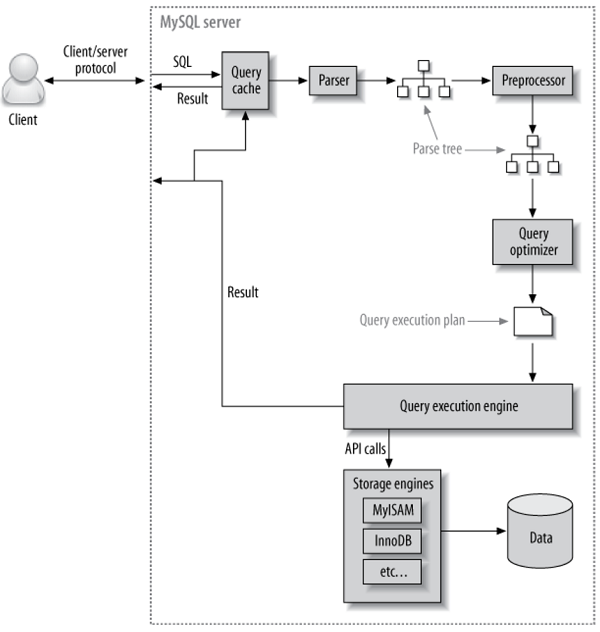
\includegraphics[angle=90,width=\textwidth]{test.png}
\end{verbatim}
\end{lined}
\caption{Example code for including \texttt{test.png} into a document.\label{figureex}}
\end{figure}
It includes the graphic stored in the file \texttt{test.png}. The
graphic is \emph{first} rotated by an angle of 90 degrees and
\emph{then} scaled to the final width of 0.5 times the width of a
standard paragraph.  The aspect ratio is $1.0$, because no special
height is specified.  The width and height parameters can also be
specified in absolute dimensions. Refer to Table~\ref{units} on
page~\pageref{units} for more information. If you want to know more
about this topic, make sure to read \cite{graphics}.

\section{Floating Bodies}
Today most publications contain a lot of figures and tables. These
elements need special treatment, because they cannot be broken across
pages.  One method would be to start a new page every time a figure or
a table is too large to fit on the present page. This approach would
leave pages partially empty, which looks very bad.

The solution to this problem is to `float' any figure or table that
does not fit on the current page to a later page, while filling the
current page with body text. \LaTeX{} offers two environments for
\wi{floating bodies}; one for tables and  one for figures.  To
take full advantage of these two environments it is important to
understand approximately how \LaTeX{} handles floats internally.
Otherwise floats may become a major source of frustration, because
\LaTeX{} never puts them where you want them to be.

\bigskip
Let's first have a look at the commands \LaTeX{} supplies
for floats:

Any material enclosed in a \ei{figure} or \ei{table} environment will
be treated as floating matter. Both float environments support an optional
parameter
\begin{lscommand}
\verb|\begin{figure}[|\emph{placement specifier}\verb|]| or
\verb|\begin{table}[|\ldots\verb|]|
\end{lscommand}
\noindent called the \emph{placement specifier}. This parameter
is used to tell \LaTeX{} about the locations to which the float
is allowed to be moved.  A \emph{placement specifier} is constructed by building a string
of \emph{float-placing permissions}. See Table~\ref{tab:permiss}.

\begin{table}[!bp]
\caption{Float Placing Permissions.}\label{tab:permiss}
\noindent \begin{minipage}{\textwidth}
\medskip
\begin{center}
\begin{tabular}{@{}cp{8cm}@{}}
Spec&Permission to place the float \ldots\\
\hline
\rule{0pt}{1.05em}\texttt{h} & \emph{here} at the very place in the text
  where it occurred.  This is useful mainly for small floats.\\[0.3ex]
\texttt{t} & at the \emph{top} of a page\\[0.3ex]
\texttt{b} & at the \emph{bottom} of a page\\[0.3ex]
\texttt{p} & on a special \emph{page} containing only floats.\\[0.3ex]
\texttt{!} & without considering most of the  internal parameters\footnote{Such as the
    maximum number of floats allowed  on one page.}, which could otherwise stop this
  float from being placed.
\end{tabular}
\end{center}
\end{minipage}
\end{table}

For example, a table could be started with the following line
\begin{code}
\verb|\begin{table}[!hbp]|
\end{code}
\noindent The \wi{placement specifier} \verb|[!hbp]| allows \LaTeX{} to
place the table right here (\texttt{h}) or at the bottom (\texttt{b})
of some page
or on a special floats page (\texttt{p}), and all this even if it does not
look that good (\texttt{!}). If no placement specifier is given, the standard
classes assume \verb|[tbp]|.

\LaTeX{} will place every float it encounters according to the
placement specifier supplied by the author. If a float cannot be
placed on the current page it is deferred either to the
\emph{figures} queue or the \emph{tables} queue.\footnote{These are FIFO---`first in first out'---queues!}  When a new page is started,
\LaTeX{} first checks if it is possible to fill a special `float'
page with floats from the queues. If this is not possible, the first
float on each queue is treated as if it had just occurred in the
text: \LaTeX{} tries again to place it according to its
respective placement specifiers (except `h,' which is no longer
possible).  Any new floats occurring in the text get placed into the
appropriate queues. \LaTeX{} strictly maintains the original order of
appearance for each type of float. That's why a figure that cannot
be placed pushes all further figures to the end of the document.
Therefore:

\begin{quote}
If \LaTeX{} is not placing the floats as you expected,
it is often only one float jamming one of the two float queues.
\end{quote}

While it is possible to give \LaTeX{}  single-location placement
specifiers, this causes problems.  If the float does not fit in the
location specified it becomes stuck, blocking subsequent floats.
In particular, you should never, ever use the [h] option---it is so bad
that in more recent versions of \LaTeX, it is automatically replaced by
[ht].

\bigskip
\noindent Having explained the difficult bit, there are some more things to
mention about the \ei{table} and \ei{figure} environments.
Use the

\begin{lscommand}
\ci{caption}\verb|{|\emph{caption text}\verb|}|
\end{lscommand}

\noindent command to define a caption for the float. A running number and
the string ``Figure'' or ``Table'' will be added by \LaTeX.

The two commands

\begin{lscommand}
\ci{listoffigures} and \ci{listoftables}
\end{lscommand}

\noindent operate analogously to the \verb|\tableofcontents| command,
printing a list of figures or tables, respectively.  These lists will
display the whole caption, so if you tend to use long captions
you must have a shorter version of the caption for the lists.
This is accomplished by entering the short version in brackets after
the \verb|\caption| command.
\begin{code}
\verb|\caption[Short]{LLLLLoooooonnnnnggggg}|
\end{code}

Use \ci{label} and \ci{ref} to create a reference to a float within
your text. Note that the \ci{label} command must come \emph{after} the
\ci{caption} command since you want it to reference the number of the
caption.

The following example draws a square and inserts it into the
document. You could use this if you wanted to reserve space for images
you are going to paste into the finished document.

\begin{code}
\begin{verbatim}
Figure~\ref{white} is an example of Pop-Art.
\begin{figure}[!hbtp]
\includegraphics[angle=90,width=\textwidth]{white-box.pdf}
\caption{White Box by Peter Markus Paulian.\label{white}}
\end{figure}
\end{verbatim}
\end{code}

\noindent In the example above,
\LaTeX{} will try \emph{really hard}~(\texttt{!})\ to place the figure
right \emph{here}~(\texttt{h}).\footnote{assuming the figure queue is
  empty.} If this is not possible, it tries to place the figure at the
\emph{bottom}~(\texttt{b}) of the page.  Failing to place the figure
on the current page, it determines whether it is possible to create a float
page containing this figure and maybe some tables from the tables
queue. If there is not enough material for a special float page,
\LaTeX{} starts a new page, and once more treats the figure as if it
had just occurred in the text.

Under certain circumstances it might be necessary to use the

\begin{lscommand}
\ci{clearpage} or even the \ci{cleardoublepage}
\end{lscommand}

\noindent command. It orders \LaTeX{} to immediately place all
floats remaining in the queues and then start a new
page. \ci{cleardoublepage} even goes to a new right-hand page.

% Local Variables:
% TeX-master: "lshort2e"
% mode: latex
% mode: flyspell
% End:
